\documentclass[12pt]{article}
\usepackage{graphicx}
\usepackage{caption}
\usepackage{subcaption}
\usepackage{longtable}
\usepackage{booktabs}
\usepackage{csvsimple}
\usepackage{geometry}

% Adjust page geometry to leave more space for captions
\geometry{bottom=1.5in}

% Improve caption spacing and style
\usepackage[font=normal,labelfont=bf,skip=10pt]{caption}
\captionsetup{belowskip=20pt} % Add significant space below captions

\renewcommand{\thefigure}{Extended Data Figure \arabic{figure}}
\renewcommand{\figurename}{}
\renewcommand{\thetable}{Extended Data Table \arabic{table}}
\renewcommand{\tablename}{}

% Add this to create a minipage environment for figures
\newenvironment{figurehere}[1][0.85]
  {\begin{figure}[p]
   \begin{minipage}[c][0.80\textheight][c]{\linewidth}
   \centering
   \setlength{\textfloatsep}{0pt}}
  {\end{minipage}
   \end{figure}}

\begin{document}
\setlength{\parindent}{0em} % Set the paragraph indentation to 1em

\vspace*{\fill}
\section*{\centering Extended Data Figures}
\vspace*{\fill}

\newpage

\begin{figurehere}
    \includegraphics[width=\textwidth]{extended_data/ED1_hirise_morphologies.png}
    \caption[Layered and massive textured feldspathic outcrops in HiRISE and CTX images.]{Layered and massive textured feldspathic outcrops in HiRISE (top left, middle, bottom left) and CTX images (top right, bottom right). The bottom right CTX image shows an example of "mega breccia" morphology, with both blocky/angular and rounded light-toned blocks surrounded by darker-toned material.}
    \label{fig:extended_data_figure1}
\end{figurehere}

\clearpage

\begin{figurehere}
    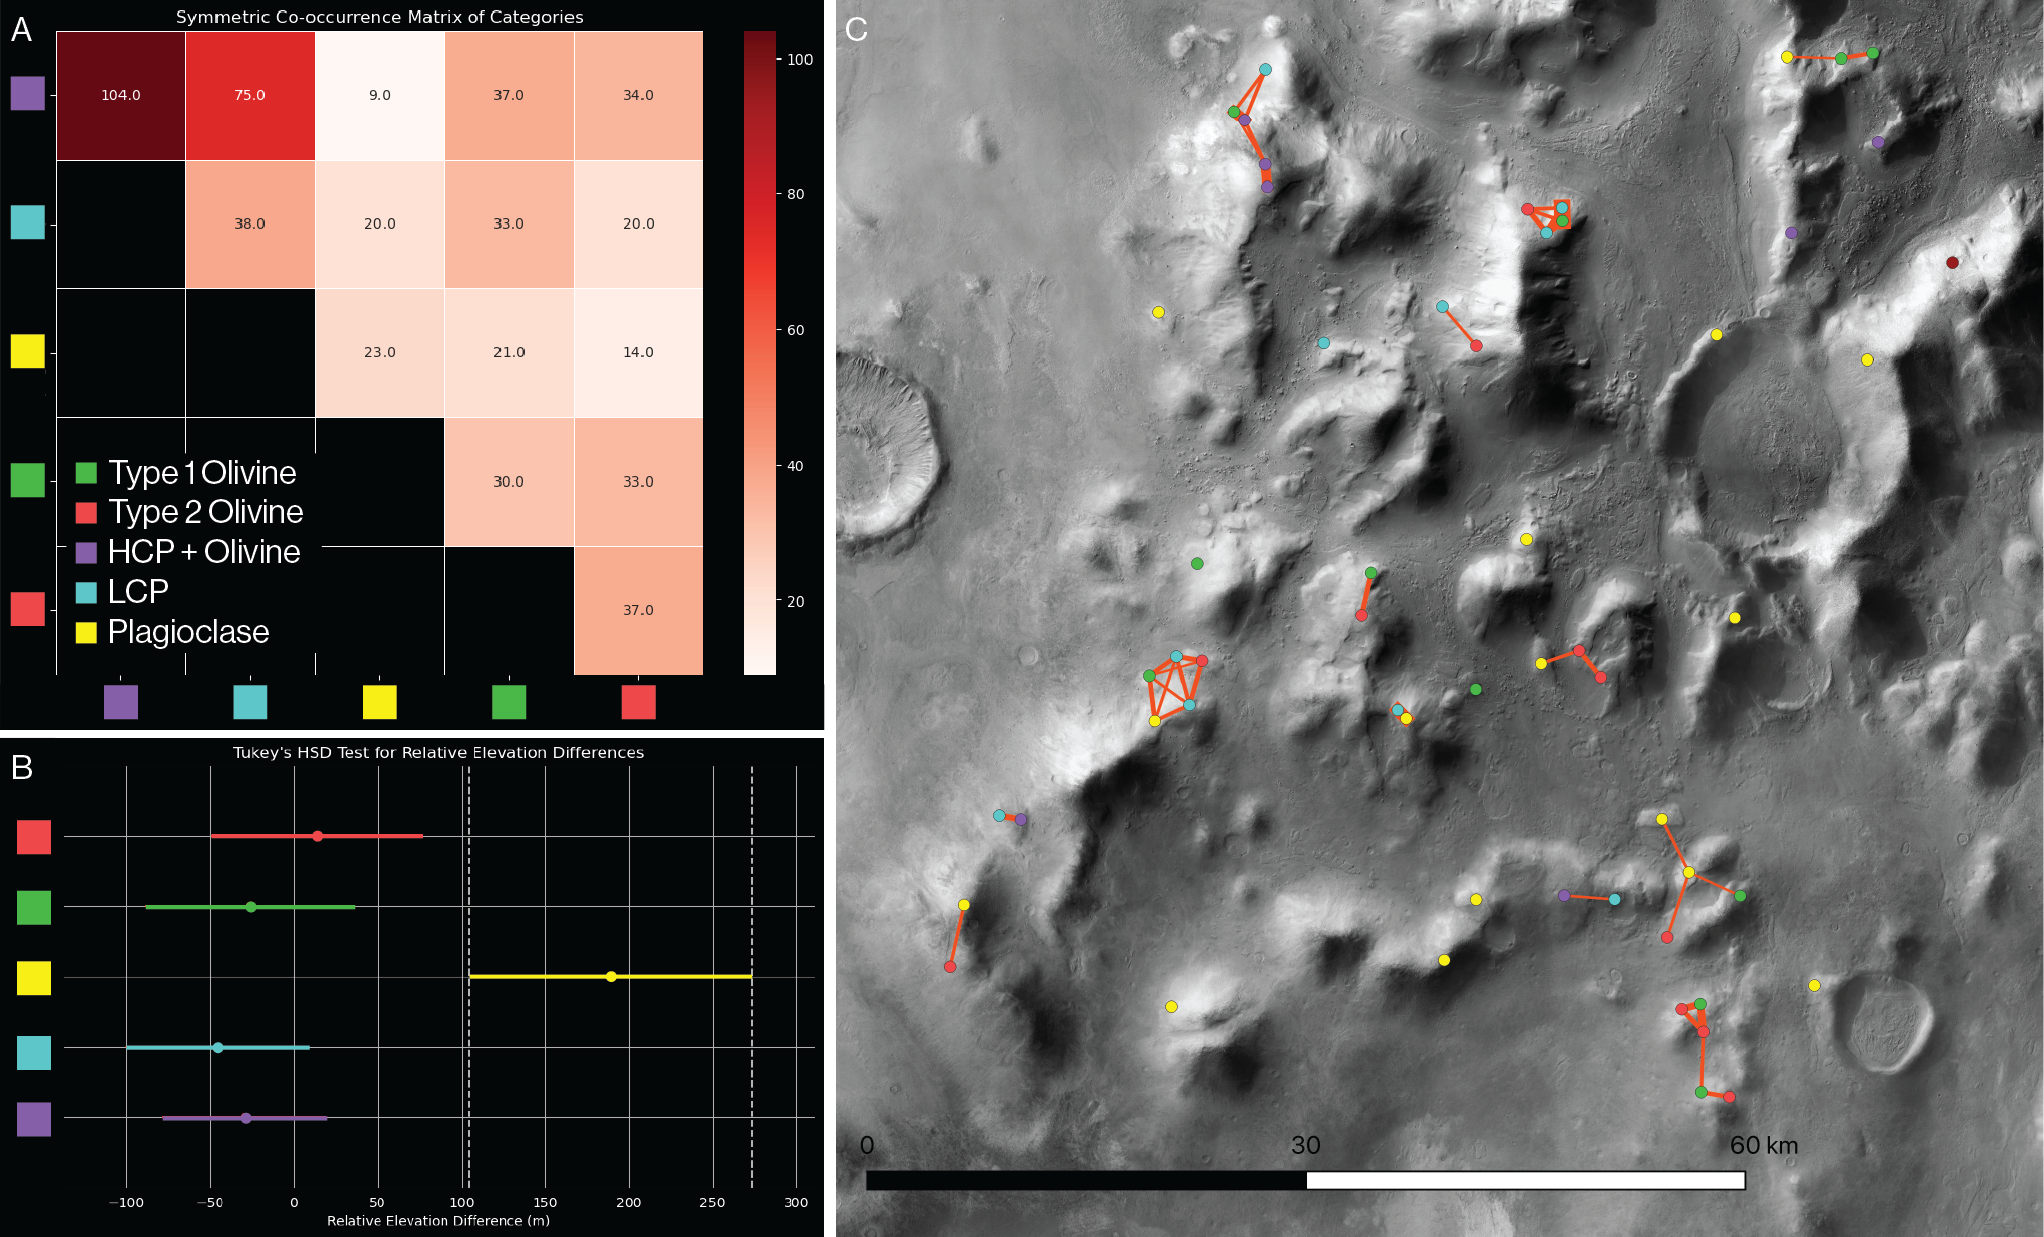
\includegraphics[width=\textwidth]{extended_data/ED2_local_relationships.png}
    \caption[Results of a graph network analysis on the local context of primary igneous minerals.]{Results of a graph network analysis on the local context ($\leq$ 5km) of primary igneous minerals surrounding the Argyre basin. A) Symmetric Co-occurrence matrix among the 5 categories of interest for this study: olivine + HCP (purple), LCP (cyan), plagioclase (yellow), type 1 olivine (green) and type 2 olivine (red). B) Results from Tukey's HSD test (performed after a one-way ANOVA) showing the relative elevation (x-axis) for each category compared to its neighbors. The 95\% confidence intervals (horizontal bars) for each category intersect zero except for plagioclase, which is approximately 200 m above its neighboring outcrops on average. C) Example connections (orange lines) among outcrops (dots) in the graph network. Line thickness is inversely proportional to outcrop distance. Dot colors correspond to the same category colors as in A and B.}
    \label{fig:extended_data_figure2}
\end{figurehere}

\clearpage

\begin{figurehere}
    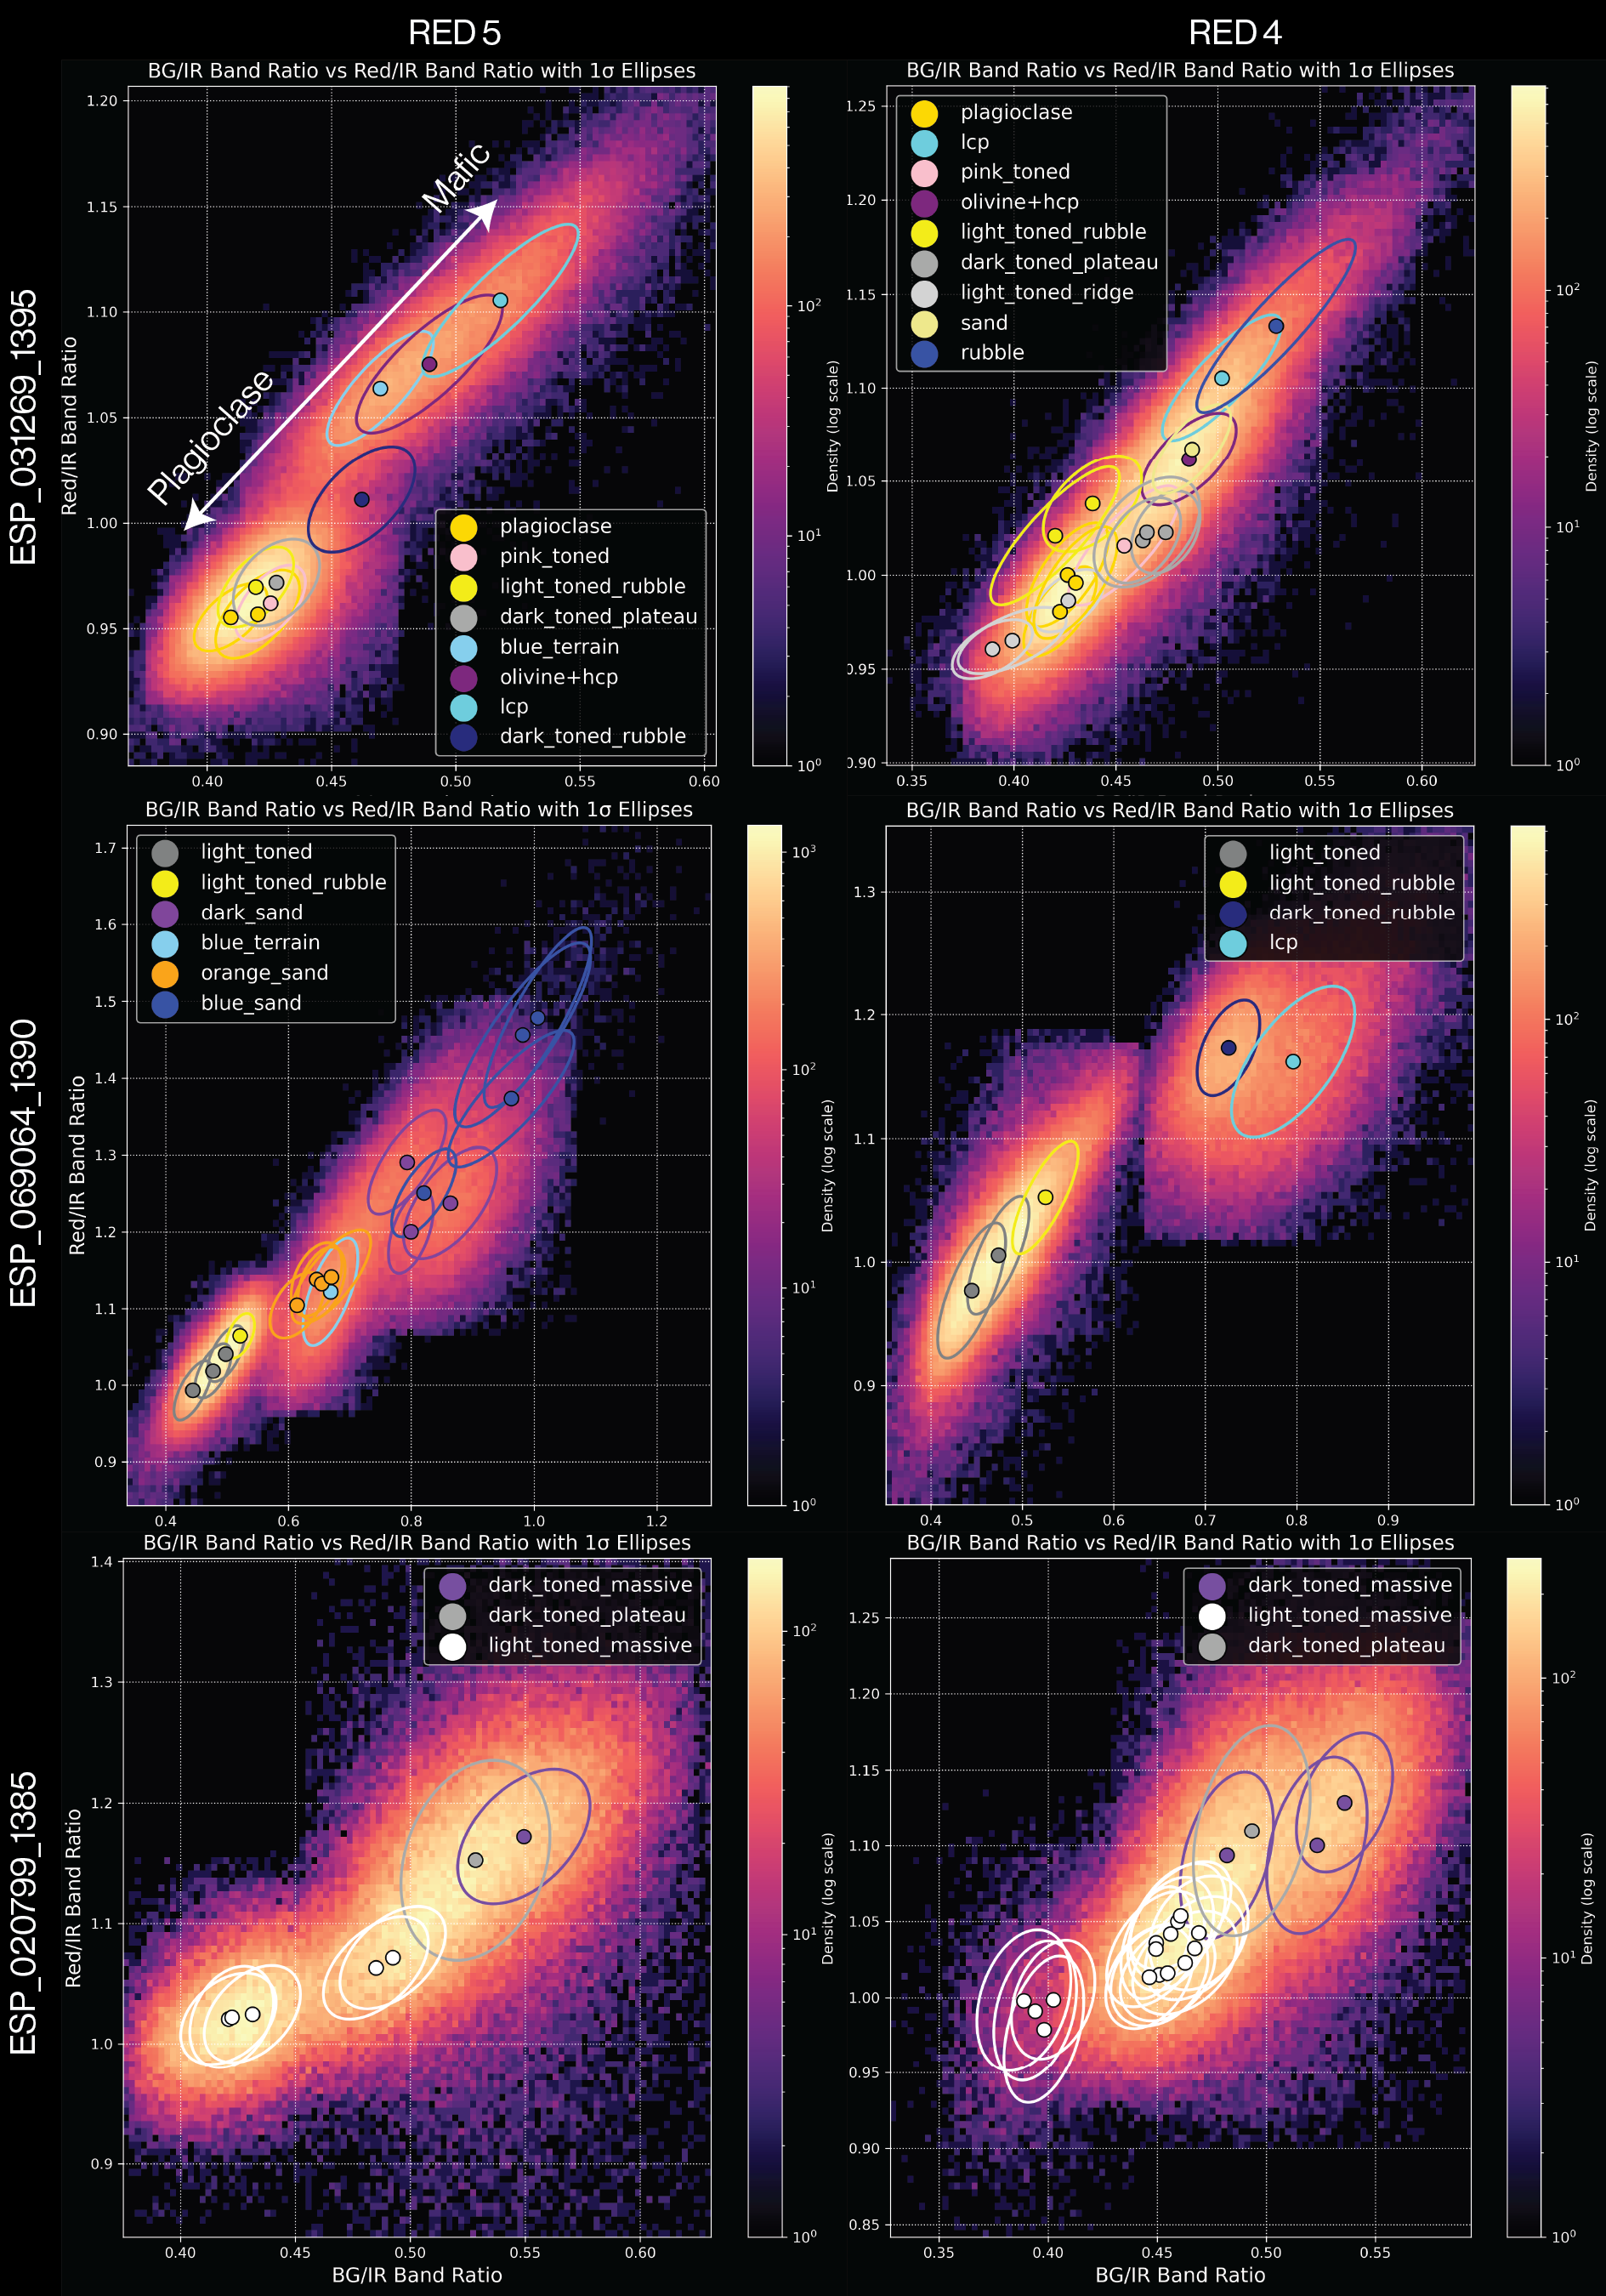
\includegraphics[width=0.9\textwidth]{extended_data/ED3_hirise_color_params.png}
    \caption[Band ratio plots for plagioclase and mafic minerals.]{Band ratio plots showing high IR/BG and IR/Red ratio values for plagioclase compared to same-scene mafic minerals.}
    \label{fig:extended_data_figure3}
\end{figurehere}

\clearpage

\begin{figurehere}
    \includegraphics[width=0.9\textwidth]{extended_data/ED4_hirise_color_images.png}
    \caption[HiRISE data and ROIs used for band ratio plots.]{HiRISE data and ROIs used to create plots in Extended Data Fig. 3.}
    \label{fig:extended_data_figure4}
\end{figurehere}

\clearpage

\begin{figurehere}
    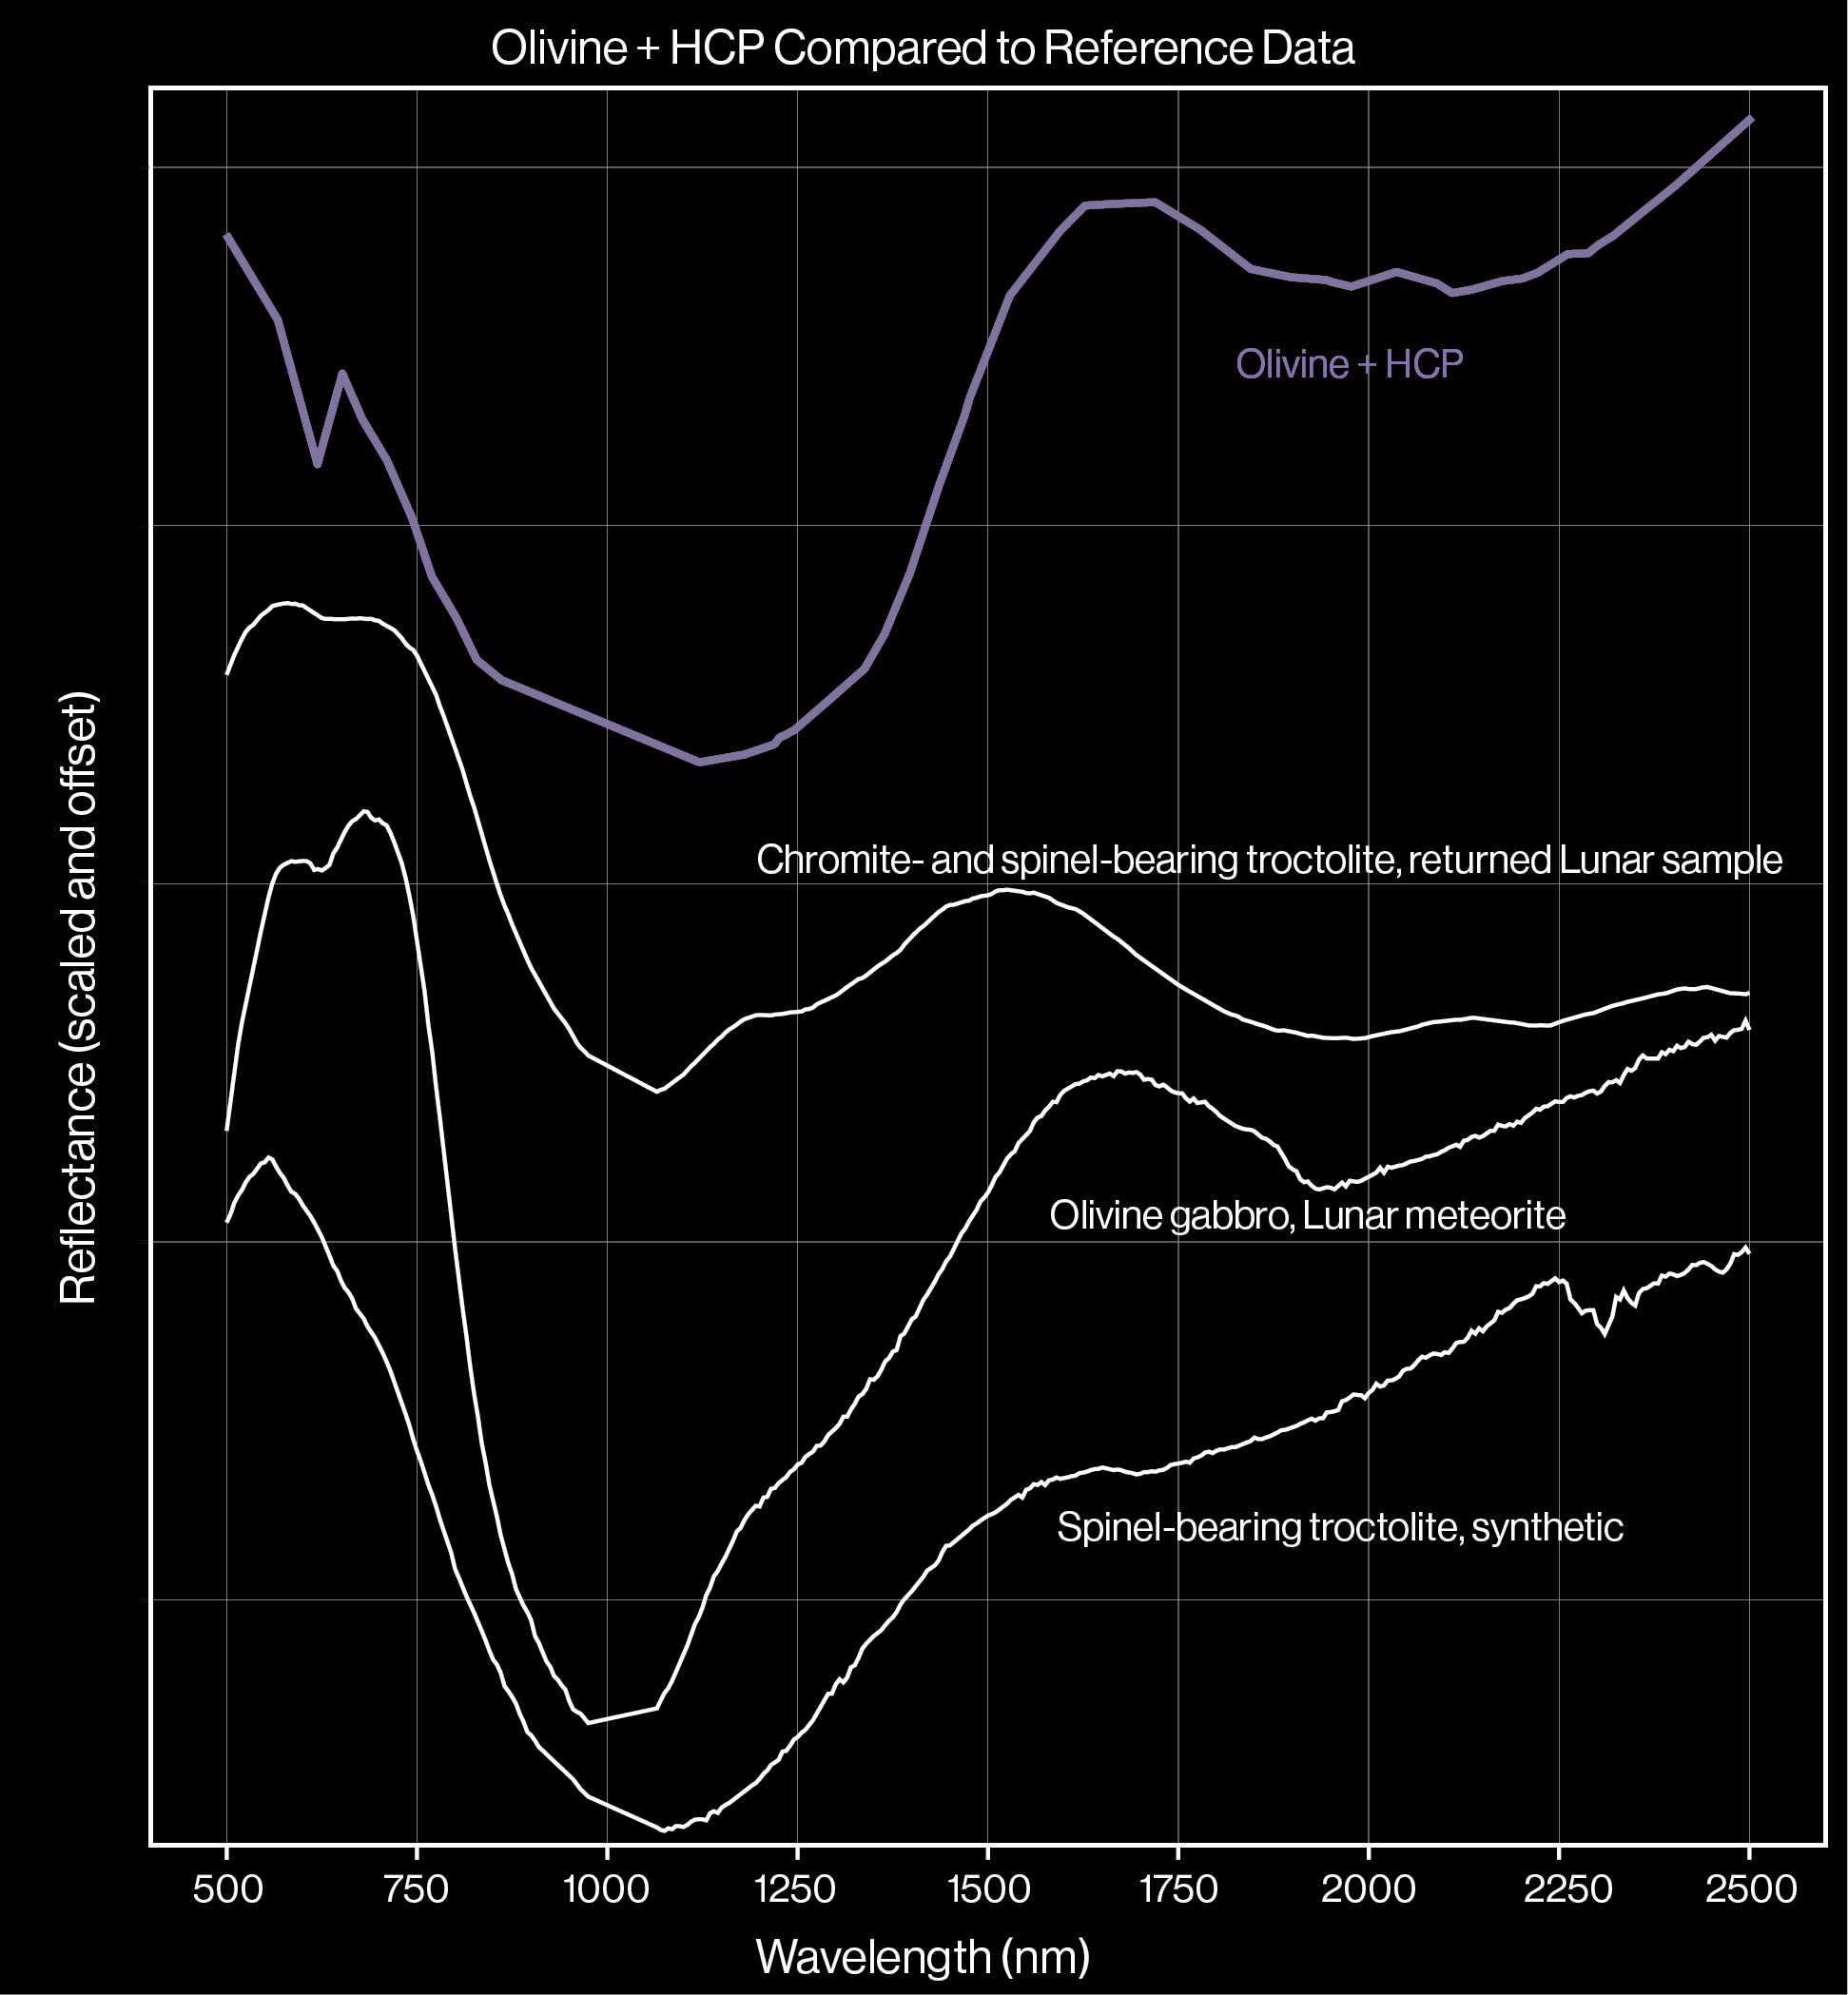
\includegraphics[width=0.9\textwidth]{extended_data/ED6_olivine_hcp_spec_fig.png}
    \caption[Comparison of Olivine + HCP category to library reference data.]{Comparison of the Olivine + HCP category to library reference data from RELAB. Our categorization label implies the lithology may be lherzolite/wehrlite/gabbro (olivine + high-calcium pyroxene ± plagioclase; compare to olivine gabbro lunar meteorite spectrum). An alternative interpretation may be chromite or spinel-bearing troctolite compositions (plagioclase + olivine + chromite/spinel). RELAB IDs used for this plot: sa2ls8 (chromite- and spinel-bearing troctolite returned lunar sample), camt313 (olivine gabbro lunar meteorite), and c1jg15 (synthetic spinel-bearing troctolite).}
    \label{fig:extended_data_figure6}
\end{figurehere}

\clearpage

\begin{figurehere}
    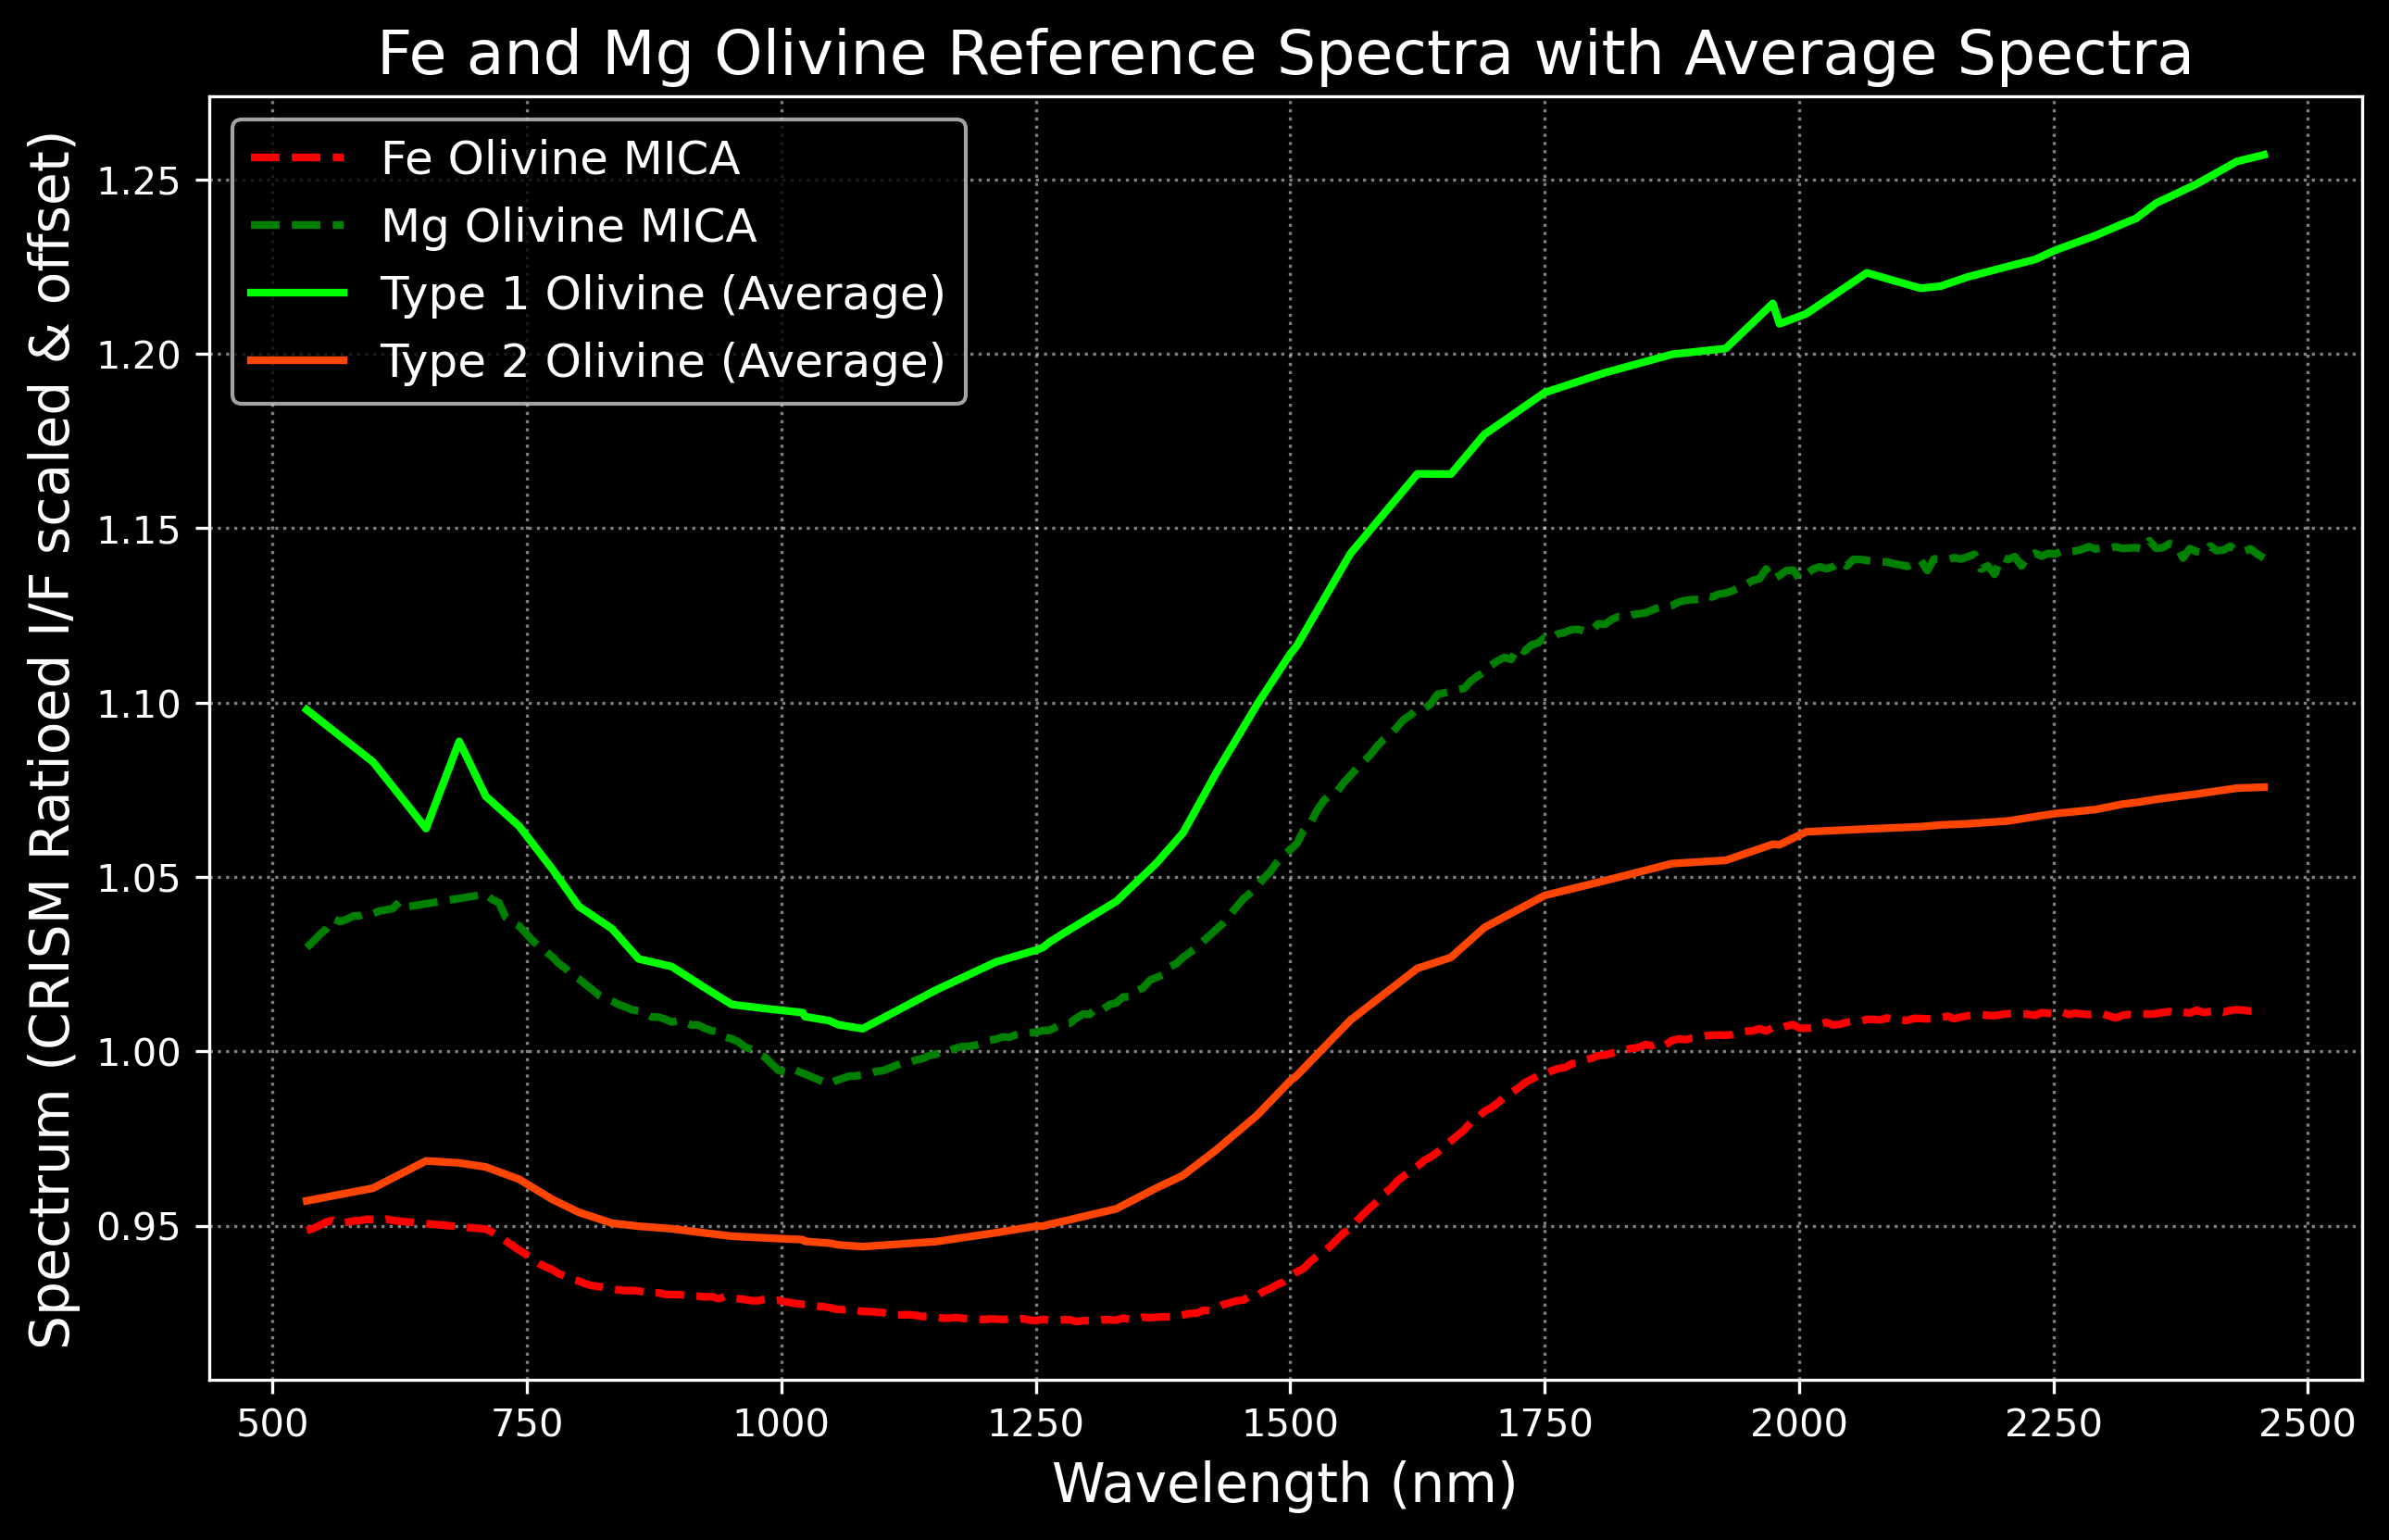
\includegraphics[width=0.9\textwidth]{extended_data/ED5_olivine_cat_spec_fig.png}
    \caption[Results from Type 1 and Type 2 olivine categorization method.]{Results from Type 1 and Type 2 olivine categorization method. Band center, band depth, slope between 1000 and 1300 nm, full width at half maximum, and band asymmetry were used to categorize the olivine detections. We performed a PCA followed by k-means clustering to assign the category labels. Dashed lines are MICA library "Mg" (green) and "Fe" (red) spectra, which correspond to Type 1 and Type 2 olivine respectively. Solid lines are the average spectra for each category attained after PCA and k-means.}
    \label{fig:extended_data_figure5}
\end{figurehere}

\end{document}

% % Extended Data Tables
% \section*{Extended Data Tables}
% \begin{longtable}{@{}llllllll@{}}
% \caption{Caption for Extended Data Table 1.} \\
% \toprule
% Tile Number & Type 1 olivine & Type 2 olivine & plagioclase & lcp & hcp + olivine & Note \\ \midrule
% \endfirsthead
% \toprule
% Tile Number & Type 1 olivine & Type 2 olivine & plagioclase & lcp & hcp + olivine & Note \\ \midrule
% \endhead 
% \csvreader[head to column names]{extended_data/ED_Table1_categorized_summary.csv}{}%
% {\\\csvcoli & \csvcolii & \csvcoliii & \csvcoliv & \csvcolv & \csvcolvi & \csvcolvii} \\
% \bottomrule
% \end{longtable}

% Add more tables as needed
% \begin{longtable}{@{}ll@{}}
% \caption{Caption for Extended Data Table X.} \\
% \toprule
% Column 1 & Column 2 \\ \midrule
% \endfirsthead
% \toprule
% Column 1 & Column 2 \\ \midrule
% \endhead
% Data X1   & Data X2   \\
% Data X3   & Data X4   \\
% \bottomrule
% \end{longtable}

\end{document}